\documentclass{article}
\usepackage{amsmath}
\usepackage{amssymb}
\usepackage{graphicx}
\usepackage{xcolor}
\usepackage{hyperref}
\usepackage{float}

\hypersetup{
    colorlinks=true,
    linkcolor=blue,
    filecolor=magenta,      
    urlcolor=blue,
    pdftitle={SAiDL Spring Assignment},
    pdfpagemode=FullScreen,
}

\title{\textbf{SAiDL Spring Assignment}}

\begin{document}

\maketitle

\section*{Disclaimer and Acknowledgements}
When I started this assignment, I didn't even know Python except \texttt{print("hello world")}. In the span of three months, I somehow managed to learn a lot of core concepts of Machine Learning. Since I had only 3 months to learn and implement everything, I had to rely on many resources.

Since I completed the assignments of the course CS231n (recommended by SAIDL), some of the setup code has been picked up from there. It was not feasible to write everything from scratch in such little time. However, I have made sure that I understand every part of the code and the math and logic behind it.

Also, one mistake that I made was not documenting the process during the project and keeping it for the end. This has caused me to forget some of the optimizations I did, but I have mentioned all the major steps involved.

\begin{center}
    \textbf{Thank You!}
\end{center}

\newpage

\section*{Core ML}

After completing a few resources, I moved on to CS231n. By the time I completed about the first four lectures, I had a basic idea of how to begin the project. I had learned two classifiers, KNN and Linear Classifier, and had no idea about CNNs. I had also learned about two loss functions, MAE and CE loss. So, I figured all I needed to do was create a linear function and instead of training the linear classifier on the original data, I had to train it after flipping the labels of 60\% of the samples. I then implemented CE, NCE, and APL loss.

Initially, I had no idea how to implement APL, but after going through some resources and reading the mentioned paper (\href{https://arxiv.org/abs/2006.13554}{Normalized Loss Functions for Deep Learning with Noisy Labels}), I identified that all I needed to do was combine two types of losses: one that punishes incorrect predictions (like CE) and one that is more lenient (like MAE).

After completing the implementation, I got very low accuracies for 60\% label noise. The accuracies were:

\begin{itemize}
    \item CE: 11.20\%
    \item NCE: 12.58\%
    \item APL: 15.96\%
\end{itemize}

Although the accuracies were very low, they revealed that APL helps avoid overfitting and improves robustness against noise.

But I was still not satisfied with the results since the paper mentioned all accuracies \textgreater 90\%. I realized that a linear classifier was too simple to achieve good accuracy. I then learned about Convolutional Neural Networks and how they could greatly improve accuracy.

\section*{Choosing CNN Implementation}
To implement a CNN, I had two choices:
\begin{enumerate}
    \item Implement a CNN using PyTorch/TensorFlow (comparatively easier)
    \item Write all the code without using any of these libraries (lengthy, time-consuming, and difficult)
\end{enumerate}

I chose the second option, despite its challenges, because I was enjoying the math behind the functions and wanted to understand what was happening inside the classes of these libraries. (I didn't realize that this was going to make the whole process very time consuming)

In \texttt{cnn.ipynb}, I implemented a CNN with the following structure:
\begin{center}
\textbf{Input \(\rightarrow\) [conv - relu - 2x2 max pool] \(\rightarrow\) affine \(\rightarrow\) relu \(\rightarrow\) affine \(\rightarrow\) softmax}
\end{center}

This basic CNN structure helped because training did not take as long as more complicated networks.

\section*{Training with No Noise}
\begin{figure}[htbp]
    \centering
    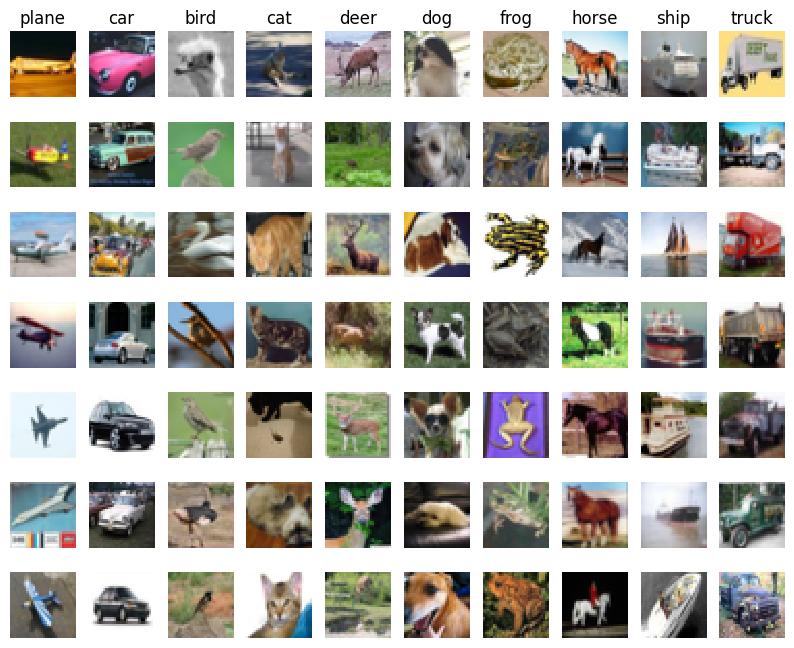
\includegraphics[width=\linewidth]{original_data.png}  % Adjust width if needed
    \caption{Original Data without noise}
\end{figure}

Initially, I trained the model without any noise using three types of losses:
\begin{itemize}
    \item Normalized Cross Entropy (NCE)
    \item Cross Entropy (CE)
    \item Active-Passive Loss (APL)
\end{itemize}

For the active part, I used CE loss, and for the passive part, I used Mean Absolute Error (MAE). After training without noise, I trained the model with 60\% label noise.

On 0-noise data:

Training accuracy with CE loss: 98.00\%

Validation accuracy with CE loss: 25.30\%

Training accuracy with NCE loss: 90.00\%

Validation accuracy with NCE loss: 25.20\%

APL Train Accuracy: 94.00\%

APL Validation Accuracy: 19.10\%

\begin{figure}[htbp]
    \centering
    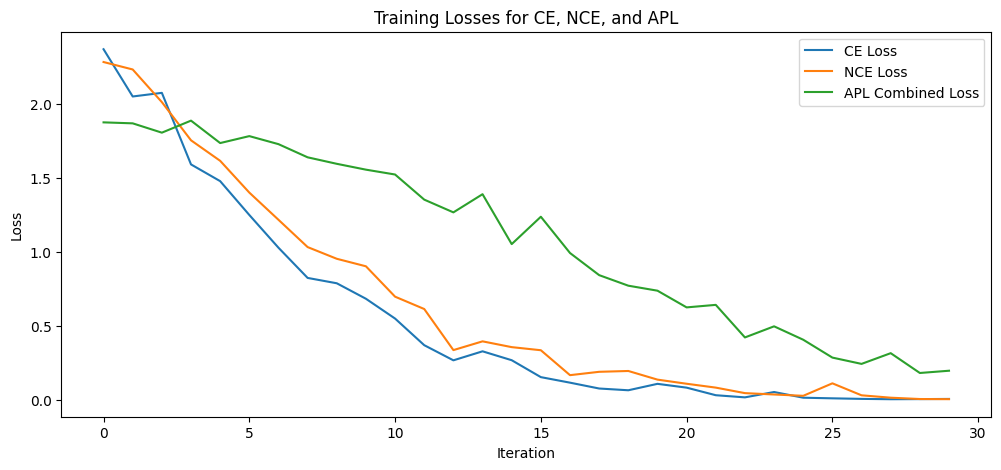
\includegraphics[width=\linewidth]{loss.png}  % Adjust width if needed
    \label{fig:your-label}
\end{figure}


\textbf{Observations:}
\begin{itemize}
    \item On training a lot of times, there was no clear winner. The fixed pattern was that validation accuracy was better for NCE \(\approx\) CE \textgreater APL, since APL “does not put as much confidence as CE and NCE”.
    \item Another pattern was that training accuracy was much higher than validation accuracy for all three. This is a classic example of overfitting. When we have too many parameters and not enough data, our model ends up overfitting, greatly affecting robustness.
\end{itemize}

\textbf{Results after Full Training:}




\begin{itemize}



    \item Available models before checking accuracy: ['ce', 'nce', 'apl']
    \item Checking accuracy for CE model:
    \begin{itemize}
        \item Training accuracy with CE loss: 46.00\%
        \item Validation accuracy with CE loss: 48.40\%
    \end{itemize}
    \item Checking accuracy for NCE model:
    \begin{itemize}
        \item Training accuracy with NCE loss: 49.00\%
        \item Validation accuracy with NCE loss: 49.30\%
    \end{itemize}
    \item Checking accuracy for APL model:
    \begin{itemize}
        \item APL Train Accuracy: 39.00\%
        \item APL Validation Accuracy: 43.40\%
    \end{itemize}
\end{itemize}

\begin{figure}[htbp]
    \centering
    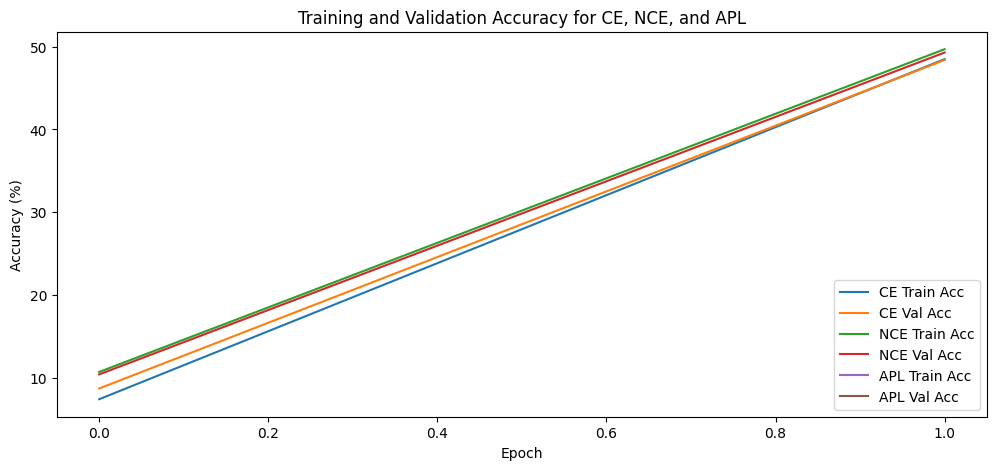
\includegraphics[width=\linewidth]{accuracies.png}  % Adjust width if needed
    \label{fig:your-label}
\end{figure}

Again, these accuracies varied a lot on training again and again and are just an example of what the accuracies looked like. 

\clearpage

\section*{Training with 0.6-Noise Data}

After adding 0.6 noise to the data, I used almost the same code as for no noise and obtained the following results:

% Place the figure here, outside the itemize
\begin{figure}[H]
    \centering
    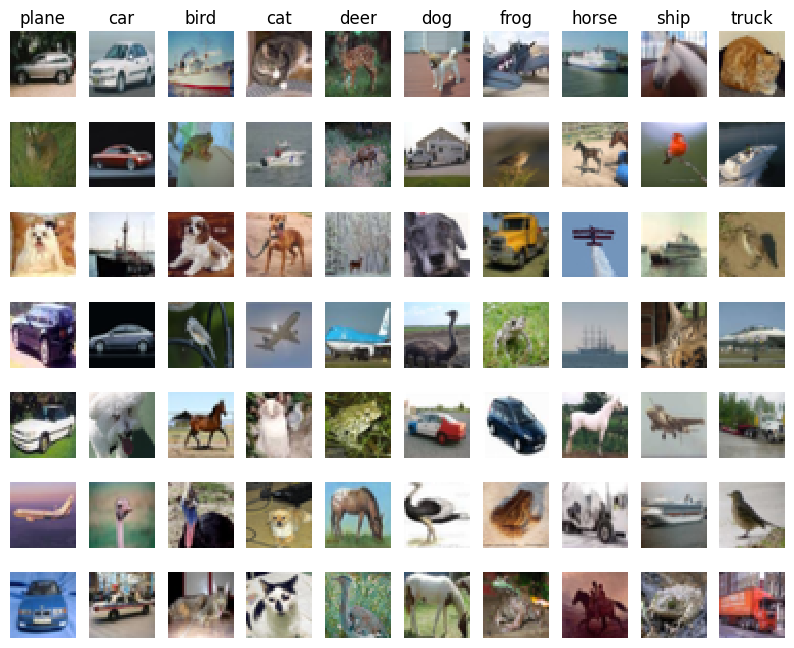
\includegraphics[width=\linewidth]{noisy_data.png}  % Adjust width if needed
    \caption{0.6 noisy data.}
    \label{fig:noisy-data}
\end{figure}
\FloatBarrier  % Ensures figure stays here before proceeding

\begin{itemize}
    \item NCE: Training accuracy: 18.00\%, Validation accuracy: 43.30\%
    \item CE: Training accuracy: 22.00\%, Validation accuracy: 41.70\%
    \item APL: Training accuracy: 23.00\%, Validation accuracy: 44.30\%
\end{itemize}

As you can see, the validation accuracies for CE and NCE loss have greatly dropped but for APL it has remained the same (if anything, it increased a bit). The results were quite consistent with the paper’s claim that the model would perform better if we use APL instead of a single loss function. This can be explained:
\begin{itemize}
    \item CE does not have any bound on the loss and tries to put all the weight on the correct class (since I used softmax to calculate probabilities).
    \item NCE, on the other hand, is slightly bounded and is not as “overconfident” as CE, and hence performs slightly better and the accuracy does not drop as much.
    \item APL performs the best of the three since it combines the “underconfident” MAE (which does not put as much weight to the correct class) and the “overconfident” CE loss.
\end{itemize}

\textbf{Note:} I was unable to get proper results for APL by coding it myself from scratch for some reason, so I had to take the help of PyTorch to implement APL (code of shame).

\begin{itemsize}
    \item I did find out that the PyTorch works and trains the code way faster than the code that I wrote in NumPy.
\end{itemsize}

\clearpage

\section*{A change in perspective}

All the documentation (pages 1-7) are from before 1st of April but since I had more time, I decided to learn PyTorch and watch the 25 hour PyTorch video tutorial in 4 days(It was very unhealthy for me lmao). I was hell-bent upon not using PyTorch, I felt like it was a cheat code but once I understood everything about PyTorch, it was like the most powerful weapon I ever had.

I implemented a very deep convolutional network following the architechture of ResNet-18. This gave me great clarity about the benefits of using APL over CE and NCE loss on noisy data. I would recommend you going through the results in 03.final.method.ipynb before reading any further.

Since we are using a very deep network, it can not only fit over normal training data, but it can also fit over noisy data. This is very evident when we view the testing accuracy of CE and NCE after about 4-5 epochs. The model begins to overfit the noisy training data and it effects its performance on testing data. 

\begin{figure}[htbp]
    \centering
    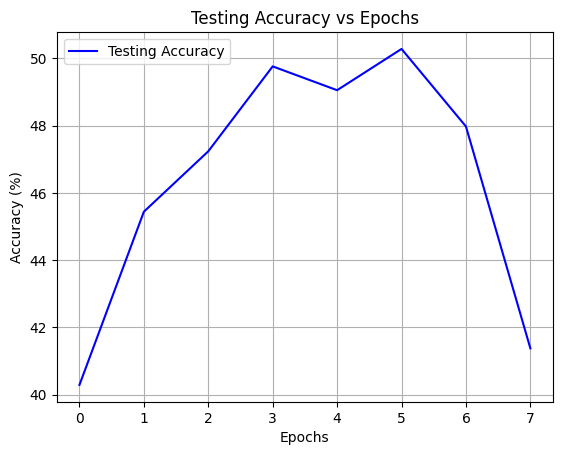
\includegraphics[width=0.7\linewidth]{nce_loss_resnet.png}  % Adjust width if needed
    \label{fig:your-label}
\end{figure}

When I trained the model using APL, I faced no such problem. Here is the comparison of CE vs NCE vs APL loss types. I have shown the performance for just 8 epochs as the compute time was going just too long and colab was disconnecting runtime.
\FloatBarrier
\begin{figure}[htbp]
    \centering
    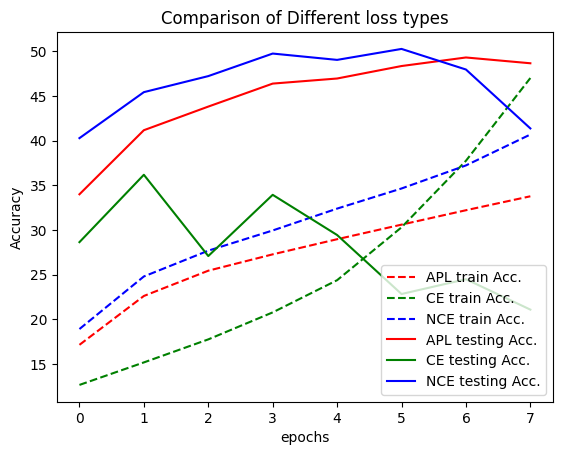
\includegraphics[width=0.7\linewidth]{comparison.png}  % Adjust width if needed
    \label{fig:your-label}
\end{figure}
\FloatBarrier

As expected, APL outperforms NCE and NCE outperforms CE loss by a margin.

\end{document}
